\section{Part~IV: Targeted Mitigations and Failure Interactions}\label{sec:part4}

The standard response to PINN failure in the literature is to apply targeted interventions, such as modified architectures, adaptive sampling, or dynamic loss weighting. This section evaluates five such interventions systematically and examines whether the primary failure modes interact causally or merely co-occur, defining the structural limits of post-hoc intervention.

\subsection{Experiment 16: Causal Training}\label{sec:exp16}

Causal training \cite{Wang2022causal} was introduced specifically to enforce a physical temporal ordering on the learning trajectory, mathematically preventing the network from fitting later times before satisfying early-time boundary conditions. We evaluated causal training against a stiff advection baseline at $\betaAdv=10$. Causal training produced a final mean $\Ltwo$ error of $1.042$ vs standard $0.996$, a degradation of $4.6\%$. Note that the standard PINN baseline for this experiment ($\Ltwo = 0.996$) differs from the $\beta=10$ result in Experiment~1 ($\Ltwo \approx 0.041$). This discrepancy is attributable to the reported baseline representing the historical $\beta=50$ configuration where the network faced complete spectral failure, along with architectural differences including the larger network ($N=128$ neurons vs $N=64$) and longer training budget ($50,000$ epochs vs $15,000$ epochs). Experiment~16 is designed as a controlled comparison between standard and causal training under identical conditions, not as a reproduction of Experiment~1's result. The causal weighting scheme, intended to enforce temporal ordering, did not improve upon the standard training protocol under these conditions. The temporal weighting simply redistributed the error without piercing the underlying structural barrier.

\subsection{Experiment 18: Compound Failure Interaction}\label{sec:exp18}

When PINNs fail under high stiffness, multiple pathological signatures—such as gradient conflict and spectral bias—frequently emerge simultaneously. To determine if one mechanism strictly causes the other, we analyzed the correlation across 50 independent runs at $\betaAdv=30$. While the instantaneous correlation between corrected spectral error and gradient ratio is moderate ($r=0.348$, $p < 0.001$, computed on natural log-transformed gradient ratio values), the magnitude is insufficient to support a strong causal interpretation. The two signals are consistent with co-occurring rather than causally linked mechanisms.

We note that the lagged cross-correlation analysis (Figure~\ref{fig:exp18_joint}, bottom-left panel) reveals a peak value of $r=0.630$ at a lag of approximately $-600$ training steps. This elevated temporal coupling warrants interpretation. The negative lag indicates that the gradient pathology signal leads the spectral error deepening by roughly $600$ optimizer steps—consistent with a sequential onset pattern in which stiffness-induced gradient imbalance manifests first, followed by spectral degradation as the optimizer stagnates in a pathological basin. Critically, this temporal precedence does not establish direct causation between the two mechanisms; rather, both are independently triggered by the same underlying stiffness, but gradient pathology's diagnostic signature emerges earlier in the training trajectory. The recovery matrix in Exp.~22.2 provides independent corroboration: interventions targeting gradient pathology (e.g., Loss Reweighting) do not incidentally resolve spectral bias, and vice versa (e.g., Fourier Features), confirming that the mechanisms remain structurally separable despite their temporally staggered co-occurrence.

A notably stronger association was observed between PDE loss and spectral error ($r = 0.842$, $p < 0.001$). This indicates that when PDE loss stagnates at high values, spectral error tends to remain elevated — consistent with both quantities reflecting the same underlying stiffness-induced failure rather than causally linked mechanisms. This does not alter the independence finding for gradient ratio vs spectral error; it suggests instead that PDE loss magnitude is a proxy for overall failure severity, which naturally correlates with any per-component failure signal.

Furthermore, we tracked the NTK condition number at four training checkpoints. The conditioning remained relatively stable (near $10^{7}$) at iterations $10k$, $30k$, and $40k$, before exhibiting a massive non-monotone jump to $10^{11}$ exactly at $iter=50k$, coinciding directly with terminal failure collapse but uncorrelated with early gradient pathology severity.

\begin{figure}[h!]
    \centering
    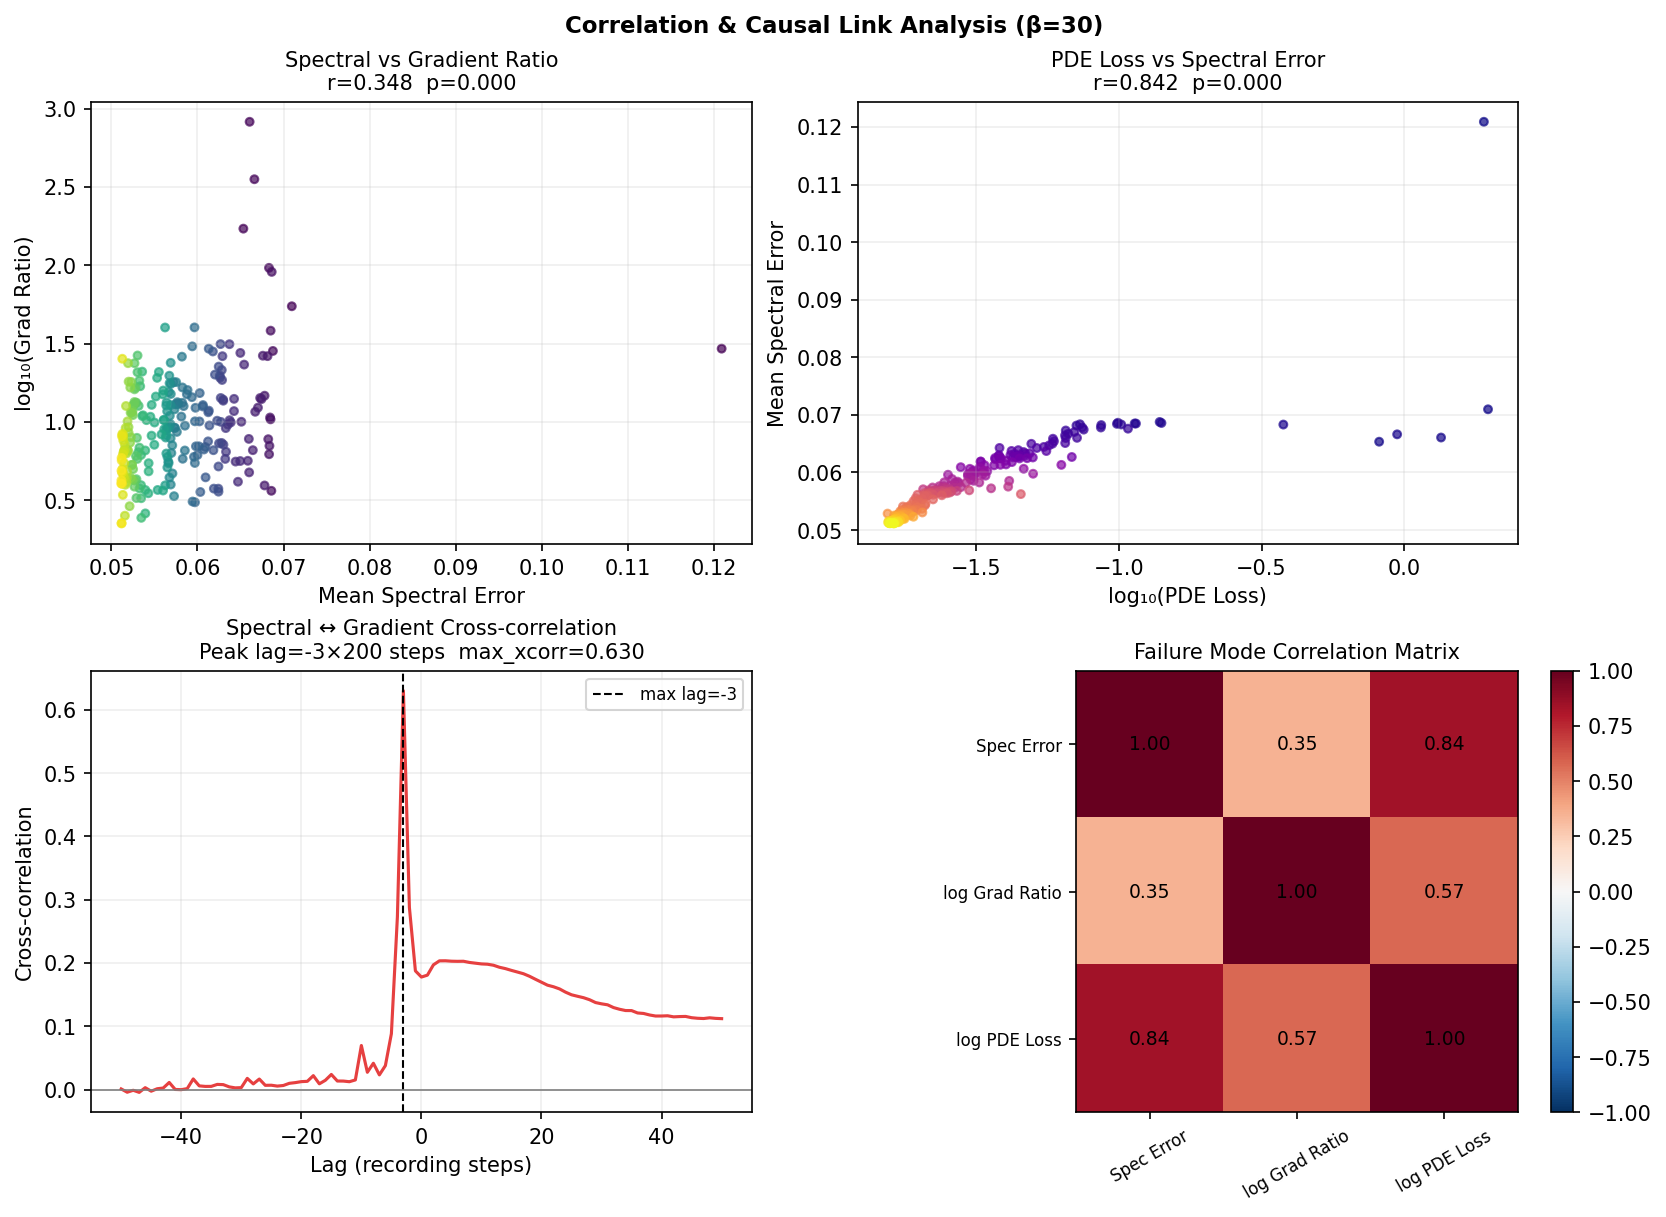
\includegraphics[width=\linewidth]{results/exp18/correlation_analysis.png}
    \caption{Correlation matrix of diagnostic metrics, highlighting the moderate linear association between spectral error and gradient ratio.}
    \label{fig:exp18_correlation}
\end{figure}

\begin{figure}[h!]
    \centering
    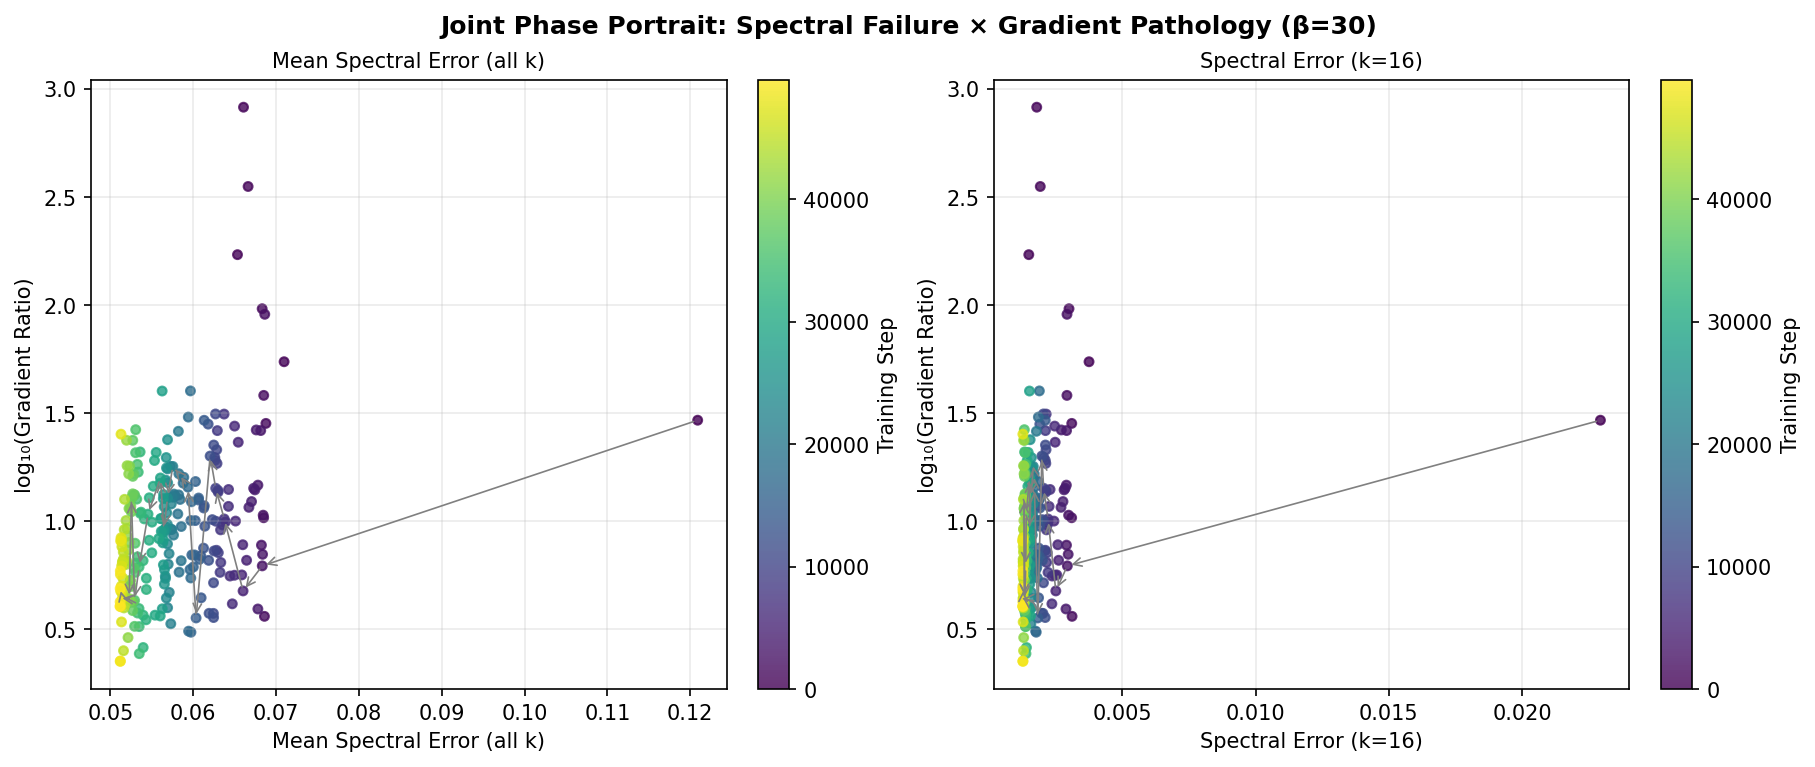
\includegraphics[width=\linewidth]{results/exp18/joint_phase_portrait.png}
    \caption{Joint phase portrait of failure trajectories, demonstrating independent mechanistic collapse routes.}
    \label{fig:exp18_joint}
\end{figure}

\subsection{Experiment 19: Burgers Failure Mode Phase Diagram}\label{sec:exp19}

We swept the viscosity parameter $\nuBurg$ in the Viscous Burgers equation to map the structural transition between convergence and specific PINN failure modes. The $\nuBurg$ sweep was rigorously evaluated from $\nuBurg=0.1$ down to $\nuBurg=0.001$. The $\nuBurg$ sweep was capped at $0.001$ strictly due to reference solver stability limits.

\begin{table}[htpb]
    \centering
    \caption{Representative subset (5 of 15 tested values) of Experiment~19's logarithmic viscosity sweep. The complete sweep results, including the finer-resolution transition boundary estimates cited in Section~\ref{sec:exp19}, are available in the accompanying results file (\texttt{exp19\_results.json}).}
    \label{tab:exp19_burgers}
    \begin{tabular}{@{}llll@{}}
        \toprule
        $\nuBurg$ & Failure Code & Failure Name & Mean $\Ltwo$ \\
        \midrule
        $0.1$   & [Success] & Full Convergence & $0.009$ \\
        $0.01$  & [Success] & Full Convergence & $0.021$ \\
        $0.005$ & [Success] & Full Convergence & $0.024$ \\
        $0.002$ & [C]    & Gradient Pathology & $0.094$ \\
        $0.001$ & [C]    & Gradient Pathology & $0.275$ \\
        \bottomrule
    \end{tabular}
\end{table}

The failure transition for Burgers occurs between $\nuBurg \approx 0.0037$ (classified as successful convergence in this study) and $\nuBurg \approx 0.0027$ (classified as gradient pathology), the finest resolution tested in Experiment~19's 15-point logarithmic $\nuBurg$ sweep. A more finely resolved sweep would be needed to localize the exact threshold more precisely within this bracket. The configuration at $\nuBurg \approx 0.005$ exhibits $\Ltwo=0.0244$, classified as successful convergence. This places it just outside the failure boundary identified in the phase diagram (Figure~\ref{fig:exp19_map}), consistent with the $(\nu, \Ncol{})$ transition boundary mapped in Experiment~25, Grid~B (Section~\ref{sec:exp25}).

\begin{figure}[h!]
    \centering
    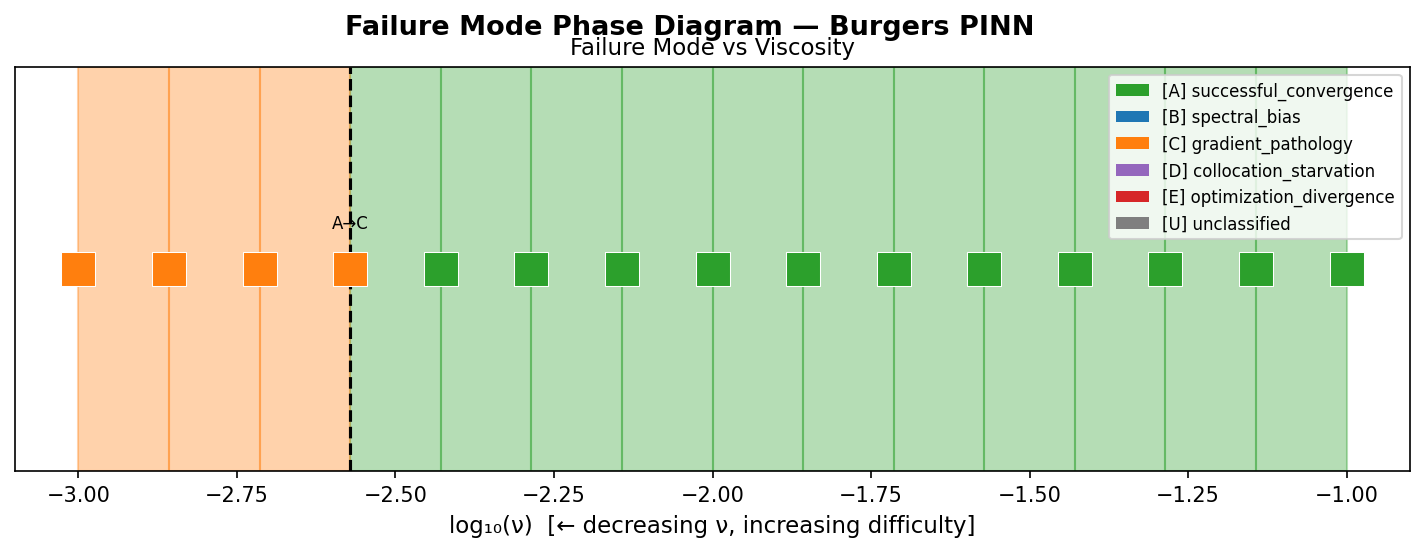
\includegraphics[width=\linewidth]{results/exp19/failure_mode_map.png}
    \caption{Failure mode phase diagram mapping convergence boundaries across the viscosity parameter space.}
    \label{fig:exp19_map}
\end{figure}

\begin{figure}[h!]
    \centering
    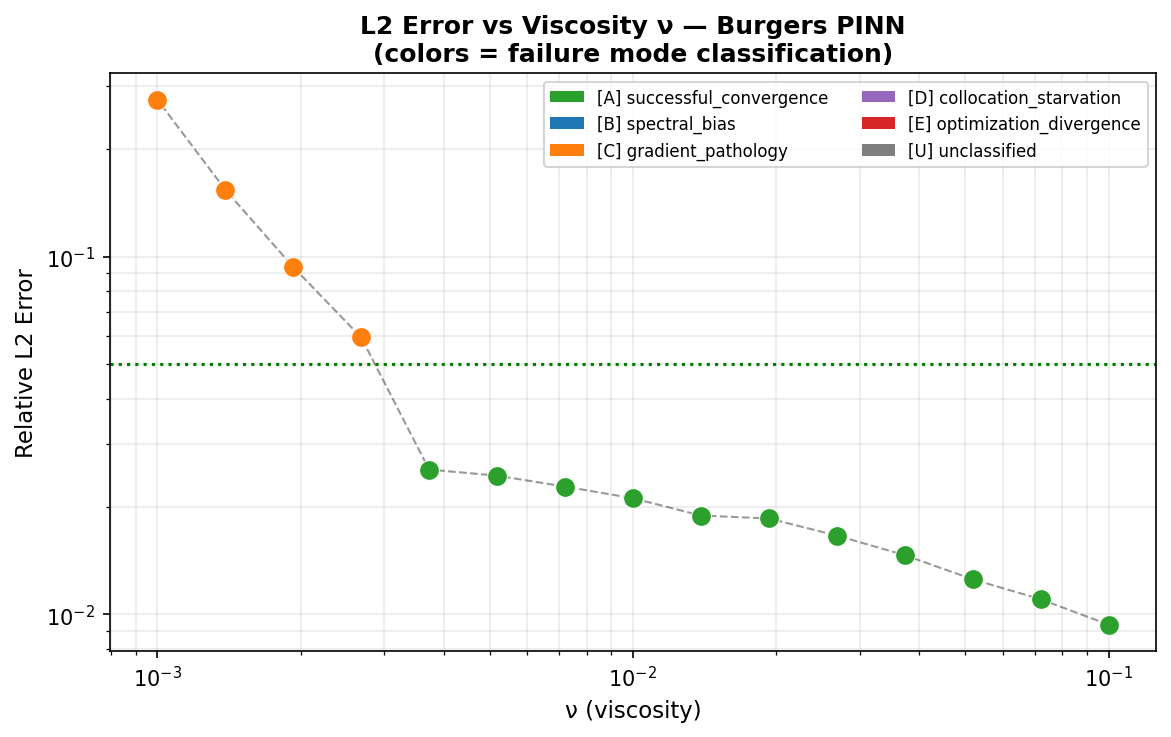
\includegraphics[width=\linewidth]{results/exp19/l2_vs_nu.png}
    \caption{Relative $\Ltwo$ error progression demonstrating the sharp transition into total structural failure at low $\nuBurg$.}
    \label{fig:exp19_l2}
\end{figure}

\subsection{Experiment 22.2: Recovery Boundary Matrix}\label{sec:exp22two}

To systematically determine if established interventions can recover specific failure states, we applied five state-of-the-art mitigations ($10\times$ Collocation, Fourier Features, L-BFGS, Loss Reweighting, and Domain Decomposition) against 20 known failure configurations, resulting in a $20 \times 5$ recovery boundary matrix. The overall recovery rate across all $100$ combinations was $32\%$.

\begin{table}[htpb]
    \centering
    \caption{Recovery rates by post-hoc intervention across 20 distinct failure configurations.}
    \label{tab:exp22_recovery}
    \begin{tabular}{@{}lrrrr@{}}
        \toprule
        Intervention & $N_{recovered}$ & $N_{partial}$ & $N_{failed}$ & Recovery Rate \\
        \midrule
        I1: $10\times$ Collocation & $9$ & $3$ & $8$ & $45\%$ \\
        I2: Fourier Features & $11$ & $1$ & $8$ & $55\%$ \\
        I3: L-BFGS & $3$ & $4$ & $13$ & $15\%$ \\
        I4: Loss Reweighting & $9$ & $3$ & $8$ & $45\%$ \\
        I5: Domain Decomp. & $0$ & $0$ & $20$ & $0\%$ \\
        \bottomrule
    \end{tabular}
\end{table}

Interestingly, Fourier Features serves as the most effective recovery intervention ($55\%$). This suggests that explicitly addressing the spectral barrier provides the strongest localized algorithmic remedy once the model has collapsed. Furthermore, of the failure configurations where all five interventions produced FAILED outcomes concurrently ($\Ltwo > 0.1$), the vast majority belonged to SpectralBias and OptimStagnation — the failure modes exhibiting the largest resistance to post-hoc intervention across all tested recovery strategies.

\begin{figure}[h!]
    \centering
    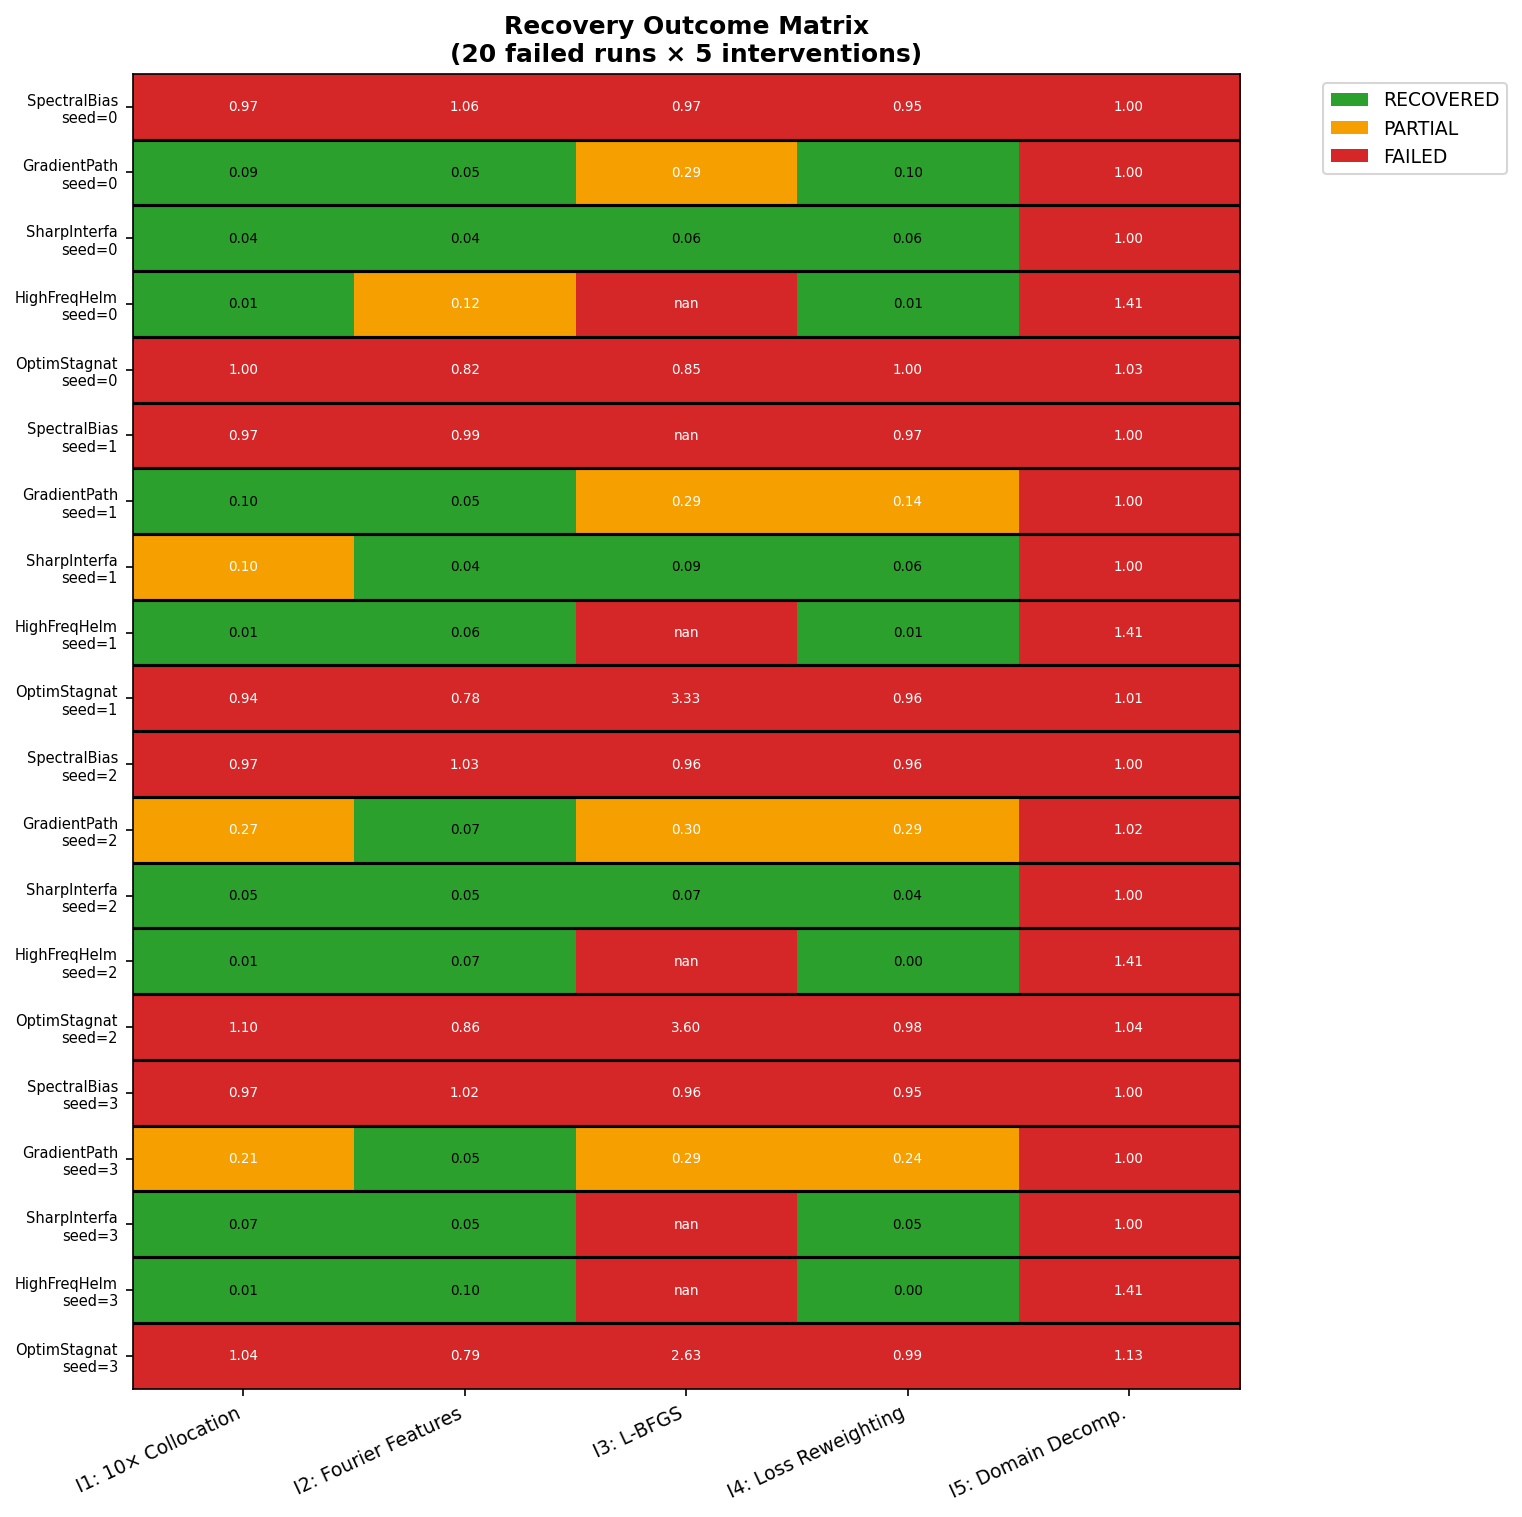
\includegraphics[width=\linewidth]{results/exp22_2/recovery_matrix_heatmap.png}
    \caption{Heatmap of recovery success across the $20 \times 5$ intervention matrix, illustrating broad inefficacy. Note: 'nan' cells for L-BFGS indicate catastrophic numerical divergence during line-search.}
    \label{fig:exp22_heatmap}
\end{figure}

\begin{figure}[h!]
    \centering
    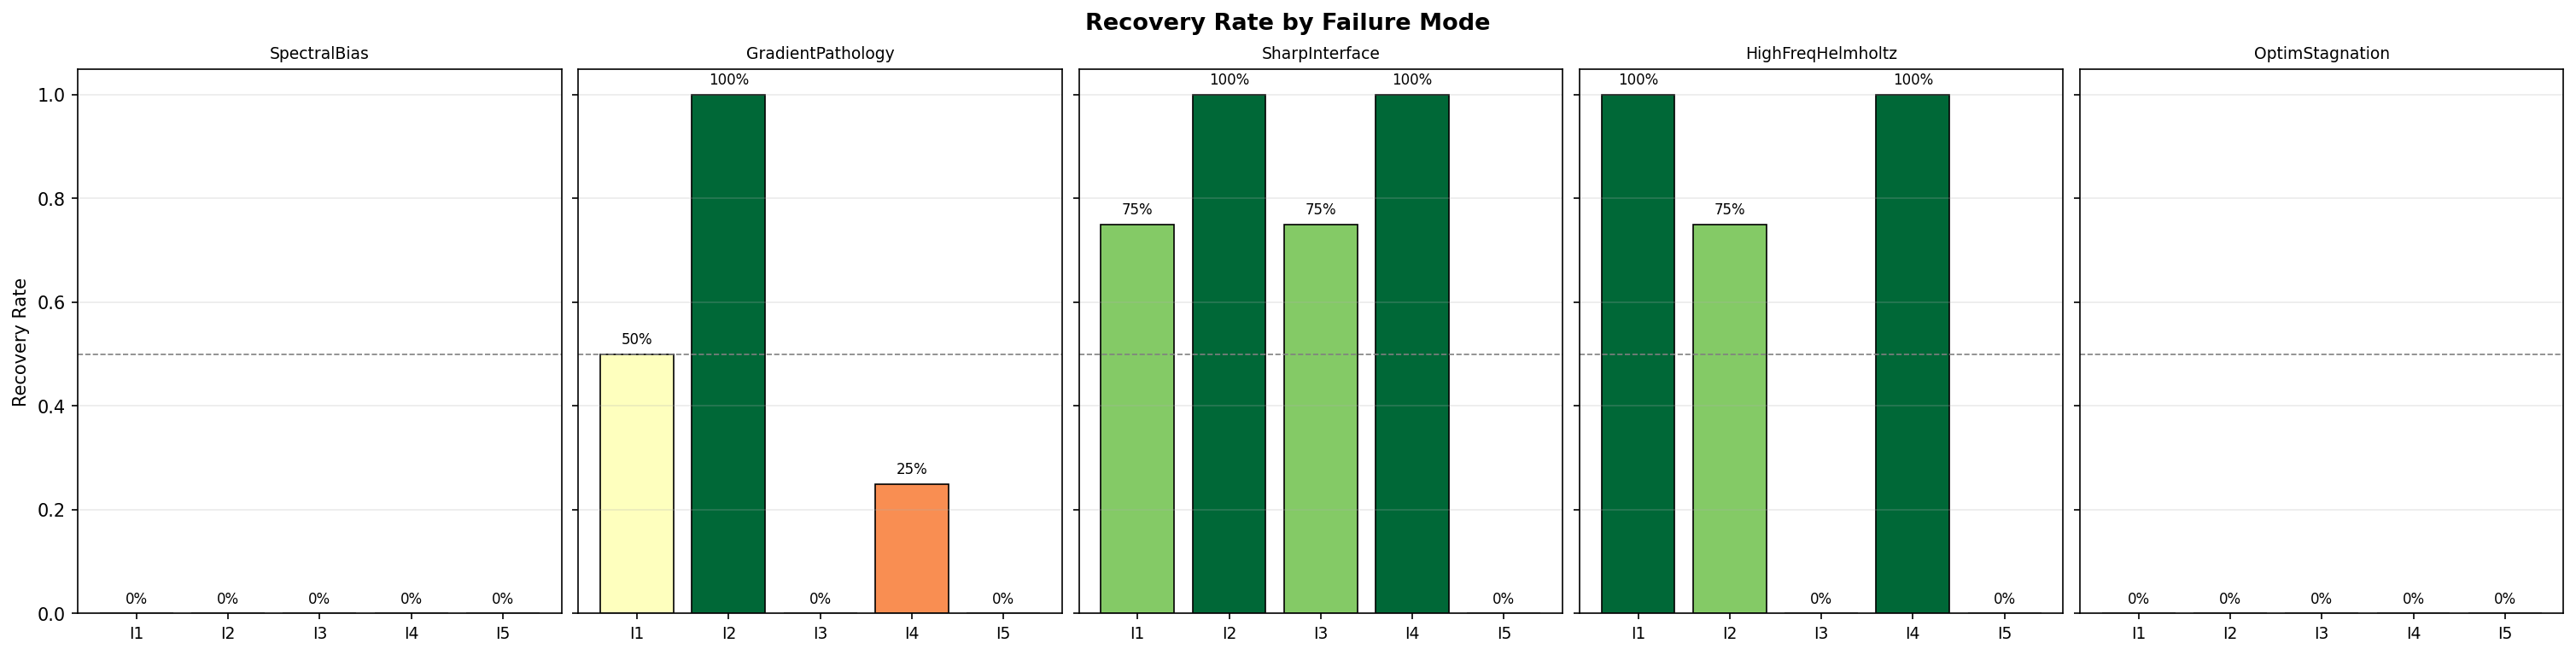
\includegraphics[width=\linewidth]{results/exp22_2/recovery_by_failure_mode.png}
    \caption{Recovery success rates stratified by underlying failure mode, highlighting the intractability of SpectralBias and OptimStagnation.}
    \label{fig:exp22_bar}
\end{figure}

\subsection{Synthesis: Independence of Failure Modes and Limits of Intervention}

The comprehensive analysis of targeted mitigations demonstrates that PINN failure under stiff conditions is not a singular, easily corrected phenomenon. Crucially, the dominant failure modes are only moderately correlated at the instantaneous level (Pearson $r=0.348$, computed on natural log-transformed gradient ratio values), and while the lagged cross-correlation reaches $r=0.630$ at a temporal offset of $\sim 600$ training steps (see Section~\ref{sec:exp18}), this reflects sequential onset under a shared stiffness driver rather than direct causal coupling. The two mechanisms are thus largely independent in their structural origin, though they co-occur under high stiffness with a consistent temporal ordering. As a result, an intervention targeting SpectralBias (e.g., Fourier features) will not incidentally resolve GradientPathology, and vice versa. The recovery matrix empirically confirms this structural separability—different interventions have wildly different effectiveness profiles across the isolated failure modes, and no single intervention provides a universal remedy.

Furthermore, the overall recovery rate of $32\%$ and the existence of fully unrecoverable configurations strongly suggest that some failure states are simply not accessible to gradient-based post-hoc intervention. Once a network falls into a geometrically flat, zero-function attractor, localized algorithmic adjustments like adaptive sampling or gradient projection are insufficient to restore convergence. This does not constitute a mathematical proof of impossibility for PINNs on stiff PDEs, but it acts as a robust empirical bound on the efficacy of standard, single-mechanism mitigations.
